\subsection{Lớp blockchain -- mạng Hyperledger Fabric riêng tư}

\subsubsection{Lý do lựa chọn Hyperledger Fabric}

Hệ thống bầu cử yêu cầu hai đặc tính trái ngược với blockchain công khai: \textbf{xác minh danh tính} của từng node và \textbf{tính chung quyết xác định} (\textit{deterministic finality}). Một mạng công khai như Ethereum không thỏa mãn cả hai -- bất kỳ ai cũng có thể tham gia mạng và trở thành node, và các khối có thể bị thay thế tạm thời bởi nhánh dài hơn (hiện tượng \textit{fork}). Hyperledger Fabric khắc phục cả hai điểm yếu này bằng kiến trúc được cấp phép (\textit{permissioned}) và cơ chế đồng thuận xác định Raft. Bảng~\ref{tab:ethereum-vs-fabric} so sánh các tiêu chí then chốt.

\begin{table}[H]
\centering
\caption{So sánh giữa blockchain công khai (Ethereum) và Hyperledger Fabric}
\label{tab:ethereum-vs-fabric}
\begin{tabularx}{\textwidth}{|L{0.25}|L{0.35}|L{0.4}|}
\hline
\textbf{Tiêu chí} & \textbf{Ethereum / Public} & \textbf{Hyperledger Fabric} \\
\hline
Quyền tham gia & Mở -- ai cũng được & Được cấp phép (\textit{permissioned}) \\
\hline
Danh tính node & Ẩn danh & Chứng chỉ X.509 do CA cấp \\
\hline
Thông lượng & 15--30 TPS (PoW) & 3000+ TPS (PBFT/Raft) \\
\hline
Độ trễ chung quyết & 6--60 giây & dưới 1 giây (\textit{deterministic}) \\
\hline
Chi phí & Phí gas & Không có (hạ tầng riêng) \\
\hline
Dữ liệu & Công khai & Riêng tư theo \textit{channel} \\
\hline
Ngôn ngữ chaincode & Solidity (EVM) & Go, Java, Node.js \\
\hline
\end{tabularx}
\end{table}

\subsubsection{Thành phần cấp phép -- MSP và X.509}

Fabric quản lý danh tính qua \textbf{Membership Service Provider} (MSP). Mỗi tổ chức tham gia mạng có một MSP riêng, được cấp phát chứng chỉ X.509 cho ba vai trò chính: \textit{Admin} (quản trị channel), \textit{Peer} (node xác nhận và lưu sổ cái), và \textit{Client} (ứng dụng gọi chaincode). Một root CA của Fabric quản lý các CA con của từng tổ chức và CA của orderer. Mọi giao dịch gửi lên mạng đều phải mang chữ ký X.509 của client; peer node xác minh chữ ký trước khi thực thi chaincode -- không có chứng chỉ hợp lệ, giao dịch bị từ chối ngay tại tầng mạng.

\subsubsection{Cô lập theo channel và chính sách xác nhận}

Toàn bộ giao dịch bầu cử được ghi trên channel \pkg{votechannel} -- một sổ cái độc lập chỉ các tổ chức được cấp phép mới có quyền đọc và ghi. Channel khác chạy trên cùng peer cũng không thấy được dữ liệu của \pkg{votechannel}. Bên cạnh đó, chaincode \pkg{VoteLedgerContract} được cấu hình với \textbf{chính sách xác nhận} (\textit{endorsement policy}) yêu cầu một số lượng tối thiểu peer xác nhận giao dịch trước khi orderer chấp nhận đóng khối -- một peer bị xâm phạm không đủ để giả mạo giao dịch.

\subsubsection{Chaincode external và bất biến của gốc Merkle}

Chaincode được triển khai ở chế độ \textit{external} thông qua \pkg{shim.ChaincodeServer}: chaincode chạy như một tiến trình độc lập, kết nối với peer qua gRPC. So với chế độ \textit{embedded} (nhúng vào peer), cách làm này cho phép cập nhật chaincode mà không phải khởi động lại peer, debug dễ dàng hơn nhờ tiến trình riêng, và cho phép mở rộng theo chiều ngang. Sau khi giao dịch \pkg{SubmitVote} được đóng khối, băm khối được tính vào khối kế tiếp -- thay đổi bất kỳ giao dịch nào trong lịch sử sẽ làm tất cả khối sau đó trở nên không hợp lệ; trong khi đó để viết lại lịch sử cần chiếm quyền điều khiển đa số peer cùng lúc. Riêng với giao dịch \pkg{CommitMerkleRoot}, chaincode còn từ chối cả hai hành vi: gọi \pkg{CommitMerkleRoot} lần hai cho cùng một bầu cử và \pkg{SubmitVote} sau khi đã commit root.

\subsubsection{Tích hợp qua Chainlaunch -- phiên đăng nhập}

Backend không trực tiếp giao tiếp với peer Fabric mà gián tiếp qua một \textit{API Gateway} của \textbf{Chainlaunch}. Chainlaunch duy trì \textbf{một pool kết nối gRPC} đến peer Fabric thay vì mở kết nối mới cho mỗi yêu cầu từ backend. Cách làm này giúp tránh chi phí thiết lập TLS lặp lại, đồng thời cho phép Chainlaunch áp dụng cân bằng tải và logic \textit{retry/circuit-breaker} ở một điểm duy nhất. Backend chỉ cần gọi REST API thông thường -- toàn bộ độ phức tạp về giao tiếp gRPC với Fabric được đóng gói tại Chainlaunch. Mô hình kết nối tổng thể được minh họa trong Hình~\ref{fig:chainlaunch-architecture}.

\begin{figure}[H]
    \centering
    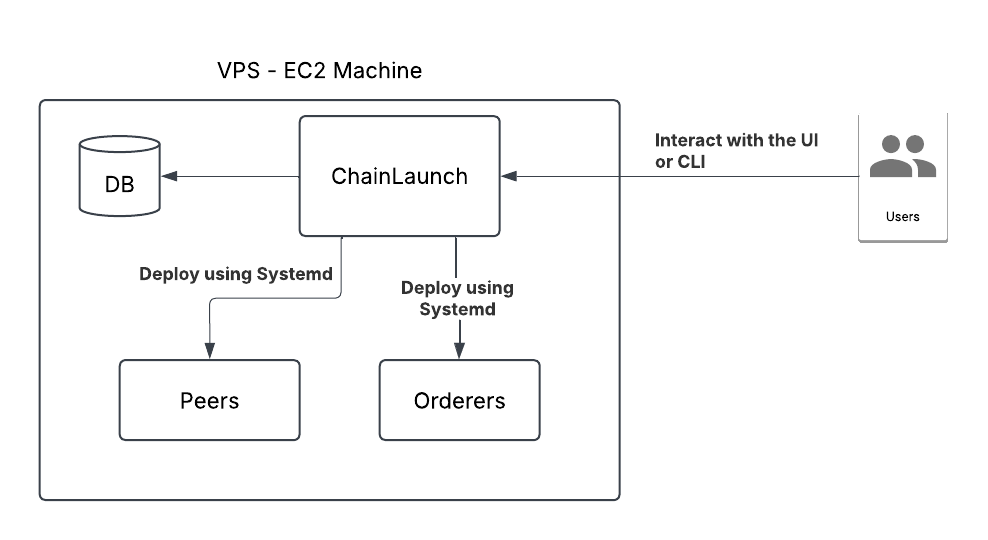
\includegraphics[width=0.85\textwidth, keepaspectratio]{Figures/Chainlaunch-architecture.png}
    \caption{Kiến trúc Chainlaunch làm cầu nối giữa backend và mạng Fabric}
    \label{fig:chainlaunch-architecture}
\end{figure}
